% @Author: AnthonyKenny98
% @Date:   2020-02-23 12:45:54
% @Last Modified by:   AnthonyKenny98
% @Last Modified time: 2020-04-05 08:04:35

\subsection{Background}
    
    The \gls{UAV} has been utilised in military applications extensively throughout the late 20th and early 21st century. However, over the last decade, their use in non-military applications, such as commerical, scientific, agricultural, and recreational, has increased such that the number of civilian drones vastly outnumber military \gls{UAV}s. \todo{cite}Particularly in the commercial sector, such rapid growth in the number and range of applications means that autonomy is key for the profitable adoption of \gls{UAV}s. Such autonomy relies on efficient computation of motion planning algorithms. However, the implementation of these algorithms can be quite computationally expensive, and thus slow and/or detrimentally power consuming. As such, this thesis aims to design specialized hardware to more efficiently compute motion plans for autonomous drones.

    \subsubsection{Autonomous Robotics}
        For well over 2000 years, the concept of robotics, albeit not always with such a term, has fascinated humans. As early as the first century A.D., the Greek mathematician and engineer, Heron of Alexandria, described more than 100 different machines and \gls{automata} in \textit{Pneumatica} and \textit{Automata} \cite{Alexandrinus}. In 1898, Nikola Tesla demonstrated the first radio-controlled vessel. Since then, the world has seen widespread application of robotics in manufacturing, mining, transport, exploration, and weaponry. For the last few decades, robots have operated in controlled, largely unchanging environments (e.g.\ an assembly line) where their environment and movements are largely known \textit{\gls{a priori}}.

        However, in recent years a new generation of autonomous robots has been developed for a wide range complex applications. These new robots are required to adapt to the changing environments in which they operate; most often, this means planning their own paths through space. As such, they must perform motion planning in \gls{real-time}.

        % % @Author: AnthonyKenny98
% @Date:   2020-02-23 12:12:56
% @Last Modified by:   AnthonyKenny98
% @Last Modified time: 2020-02-23 13:56:51

\begin{figure}%[H]
\begin{center}
\missingfigure[figwidth=\linewidth]{Some sort of line/bar graph showing the increasing use of Autonomous robots over time. Need to find}
% 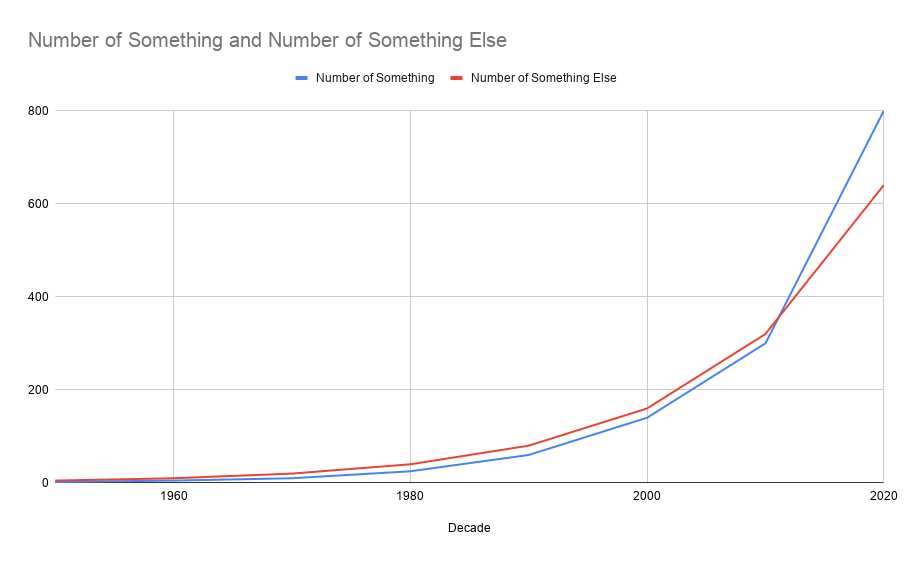
\includegraphics[width=0.8\linewidth]{img/sampleLineGraph.png}
\caption{The use of Autonomous Robots over time}
\label{fig:useOfAutonomousRobots}
\end{center}
\end{figure}

    \subsubsection{Motion Planning}
        
        While most creatures in the animal kingdom find it relatively easy to navigate their surroundings, autonomous robots must be taught explicitly how to do so by their programmers. Motion Planning refers to the problem of algorithmically determining a collision-free path between two points in an obstacle-ridden space. Chapter \ref{chap:MotionPlanningInSoftware} provides a detailed explanation of motion planning and of \glsfirst{RRT}, a commonly used motion planning algorithm.

        On the algorithmic and software level, motion planning has been extensively studied and optimized. Even so, current software implementations running on regular \glspl{CPU} are too slow to execute in \gls{real-time} for robots to operate in rapidly chainging, high complexity environments. More powerful, highly parallelized \glspl{GPU} can be used in tethered robot applications (e.g.\ robotic arms autonomously executing pick-and-place functions). However, such \glspl{GPU} consume far too much power to be used in autonomous drones, which are untethered and must sustain flight for useful periods of time. (A typical \gls{CPU} uses between 65-85 watts, while some \glspl{GPU} can use up to 270 watts\todo{cite}).

        
    \subsubsection{Application Specific Processors}

        Given the lacking performance in computing motion plans of a \gls{CPU}, and the untenable power consumption of a \gls{GPU}, autonomous drone developers are left with the option of developing an \gls{ASP}, optimized for motion planning.

        However, designing a functional, high performance processor from scratch is no small task. It requires expertise in a variety of disciplines (compilers, digital logic, operating systems, etc), and an extradordinary amount of time and effort to develop and verify before it can be used. In short, it's an expensive process, which is why the market for computer processors is dominated by companies like Intel, AMD, and ARM. The sharing of processor designs is also not possible, as commercial designs are proprietary and competing designs are not encouraged.

        Finally, even if one were to design an \gls{ASP} from scratch, or build off an existing commercial design (which means paying royalties), the \glsfirst{ISA} that the processor implements are not designed for are not designed for extendability, meaning that even a highly specialized processor is limited to a small number of instructions.

        \todo[inline]{Discuss Moore's law and denard scaling}

    \subsubsection{RISC-V}
        RISC-V (pronounced ``risk-five'') is an \gls{ISA} developed by the University of California, Berkeley. It is established on the principles of a \gls{RISC}, a class of instruction sets that allow a processor to have fewer \gls{CPI} than a \gls{CISC} (x86, the \gls{ISA} on which macOS and linux operating systems run, is an example of a \gls{CISC} instruction set). 

        What makes RISC-V unique is its open-source nature. RISC-V was started with the philosophy of creating a practical, open-source \gls{ISA} that was usable in any hardware or software without royalites. The first report describing the RISC-V Instruction Set was published in 2011 by Andrew Waterman, Yunsup Lee, David A. Patterson, and Krste Asanović \cite{Isa2012}.
    

\newpage
\subsection{Problem Definition}

    \subsubsection*{Problem Statement}
    Motion planning algorithms implemented in software that runs on general purpose \gls{CPU}s cannot execute quickly enough for fully autonomous \gls{UAV}s to operate in high-complexity environments. The state-of-the-art strategy of using power-hungry \gls{GPU}s to accelerate the execution of these algorithms requires too much power to be cost-effective or feasible for \gls{UAV}s to sustain flight for useful periods of time. \todo[size=\small, inline, caption={Improve Problem Statement}]{Existing research into accelerating robotic motion planning is <reason for RISC-V, inaccessable?> and mainly focussed on tethered arm moveing robots.}

    \subsubsection*{End User}
    This thesis aims to provide developers of autonomous drones with specialized hardware for motion planning. Such developers have a need for computing hardware that executes motion planning algorithms faster and more power efficiently than existing methods. This thesis will provide a processor design that is synthesizable on an \gls{FPGA}, giving developers a processer for which a \gls{RTOS}, or bare metal code, can be deployed.
    \todo[inline]{Revise End User}